%%%%%%%% Draft in the ICML 2027 format. Contribution type (selected on OpenReview, not in the PDF): General.
%%%%%%%% Terminology follows writeup/glossary.md: use its terms, not their synonyms.
\documentclass{article}

% Tectonic compiles with XeTeX, whose default encoding has no Times; T1 makes the style's times package apply
\usepackage[T1]{fontenc}

\usepackage{microtype}
\usepackage{graphicx}
\usepackage{booktabs}
\usepackage{hyperref}
\newcommand{\theHalgorithm}{\arabic{algorithm}}
\usepackage{icml2027}
\usepackage{amsmath}
\usepackage{amssymb}
\usepackage{mathtools}
\usepackage[capitalize,noabbrev]{cleveref}
\usepackage{pgfplots}
\pgfplotsset{compat=1.18}
\usepgfplotslibrary{groupplots}

\newcommand{\bok}{best-of-$K$}
\newcommand{\Bok}{Best-of-$K$}
\newcommand{\Y}{|Y(x)|}

\icmltitlerunning{Validity and Diversity of Recursive Reasoning Models}

\begin{document}

\twocolumn[
  \icmltitle{A Narrow Band: Measuring Validity and Diversity of\\Recursive Reasoning Models on Problems with Many Solutions}

  \begin{icmlauthorlist}
    \icmlauthor{Anonymous Authors}{anon}
  \end{icmlauthorlist}
  \icmlaffiliation{anon}{Anonymous Institution}
  \icmlcorrespondingauthor{Anonymous Authors}{anon@anon.org}
  \icmlkeywords{recursive reasoning, latent variable models, multiple solutions, posterior collapse, evaluation}
  \vskip 0.3in
]

\printAffiliationsAndNotice{}

\begin{abstract}
Many reasoning problems have more than one solution, and a model that solves them should be able to produce those
solutions, not just one. GRAM, a generative recursive reasoning model, adds stochastic guidance to a tiny recursive
network for this purpose: a random vector drawn at every transition, from a posterior that sees the target during
training and from a learned prior at test time, with a KL term of weight $\beta$ between the two. We build four puzzle
benchmarks whose solution sets are enumerated exactly, with at most 16 solutions stored per training input so that the
others are unseen solutions, and an evaluation that separates validity from diversity. We use it to compare GRAM with
a simpler baseline whose stochastic guidance never sees the target: a standard-normal prior trained with a
best-of-$K$ objective. At the authors' $\beta$, GRAM's distinct@100 is 1.2--3.3$\times$ the baseline's on three of
four tasks, but its validity is lower on all four. Its usable $\beta$ is a narrow band: halving or doubling $\beta$
degrades every task, through prior--posterior mismatch below the band and posterior collapse above it, and a $\beta$
carried over from other tasks misses the band. Posterior sampling, which draws GRAM's stochastic guidance from its
posterior at test time, separates the two failures: below the band the network still decodes valid answers, so the
prior is at fault. State noise, Gaussian noise added to the baseline's high-level state at test time, raises its
distinct@100 2.7-fold on Sudoku at
unchanged validity, but it stays below GRAM's on the two tasks with the most solutions. Both models produce unseen
solutions at the rate a uniform sampler would. This is a work in progress; the main results are from one seed, and
second seeds on Sudoku and mazes agree within 5 points.
\end{abstract}

\section{Introduction}

A Sudoku with few clues, a maze with loops or a partially filled N-Queens board has many solutions. Recursive reasoning
models such as HRM~\cite{wang2025hrm} and TRM~\cite{jolicoeur2025trm} solve most puzzles that have a unique solution,
but they are deterministic: one input, one answer. GRAM~\cite{baek2026gram} makes TRM generative by adding stochastic
guidance $\epsilon_t$ to the high-level state at every transition. During training $\epsilon_t$ is drawn from a
posterior $q_\phi(\epsilon_t\mid u_t,y)$ that sees the target $y$; at test time it is drawn from a learned prior
$p_\theta(\epsilon_t\mid u_t)$, and a KL term with weight $\beta$ ties the two together. This is the conditional VAE
recipe~\cite{sohn2015cvae}, with its known risks: if $\beta$ is too small, the posterior encodes the target in
stochastic guidance that the prior does not produce at test time; if it is too large, the posterior matches the prior
and the stochastic guidance carries nothing (posterior collapse~\cite{bowman2016generating}). GRAM's authors set
$\beta$ separately for every task.

We ask three questions about this model. \textbf{Q1:} how should $\beta$ be chosen for a new problem? \textbf{Q2:} is
drawing the stochastic guidance from a posterior that sees the target necessary during training, or can a model whose
stochastic guidance never sees the target do as well? \textbf{Q3:} does a model trained on some solutions of an input
produce its unseen solutions? Answering them needs problems where every solution is known, metrics that do not confuse
validity with diversity, and a baseline without a posterior. This paper describes the evaluation we built and the
first results.

\paragraph{Contributions.}
\begin{itemize}
  \item Four multi-solution benchmarks (mazes, 10-Queens completion, Sudoku, graph 3-colouring) with exact numbers of
  solutions from 1 to over 900, controlled mixes of unique-solution and multi-solution inputs, at most 16 stored
  solutions per training input, and a validation split for every choice made from results (\cref{sec:data}).
  \item An evaluation protocol that reports validity and diversity separately, against a uniform sampler, and shows
  why the ratio to uniform misleads when validity differs (\cref{sec:metrics}).
  \item A comparison of GRAM at its authors' $\beta$ with a posterior-free \bok{} baseline at matched compute, a
  $\beta$ sweep on all four tasks and an unseen-solution analysis (\cref{sec:results}), with ablations in
  \cref{app:extra}.
  \item Two test-time measurements that need no retraining: posterior sampling, which tells the two failures of
  $\beta$ apart, and state noise, which shows how much diversity the baseline gains without a posterior
  (\cref{sec:noise,sec:band}).
\end{itemize}

\section{Benchmarks}
\label{sec:data}

Every input's solution set $Y(x)$ is enumerated exactly (dynamic programming over BFS layers for mazes, backtracking
elsewhere). Each task has a knob that moves the number of solutions $\Y$ from 1 to hundreds, and inputs are drawn until
every group of solution counts has its quota: a third of the inputs are unique-solution inputs and the rest are spread
evenly over 2--3, 4--15, 16--63, 64--255 and 256+ solutions (N-Queens keeps its natural distribution). A training input
stores at most 16 of its solutions, drawn uniformly; the others are unseen solutions, which Q3 measures. Test and
validation inputs are new inputs from the same generators, checked to share no input with training (\cref{tab:data}).

\begin{table}[t]
\centering\small
\setlength{\tabcolsep}{3pt}
\begin{tabular}{@{}lllrr@{}}
\toprule
Task & Input & Knob & $\Y$ & Len. \\
\midrule
Maze & 15$\times$15 grid & walls removed & 1--924 & 225 \\
N-Queens & 10$\times$10 board & queens given & 1--93 & 100 \\
Sudoku & 9$\times$9 grid & clues & 1--1024 & 81 \\
Graph col. & 10 nodes & edge density & 1--9842 & 55 \\
\bottomrule
\end{tabular}
\caption{Benchmarks. A valid answer is a shortest path, a non-attacking completion, a completed grid, or a proper
3-colouring (counted up to relabelling). Maze, Sudoku and graph colouring have 100k training, 1k validation and 2k
test inputs; N-Queens has all 43{,}420 partial boards with 7--9 queens removed, split 36{,}907 / 1{,}000 / 5{,}513.
Details in \cref{app:data}.}
\label{tab:data}
\end{table}

\section{Evaluation}
\label{sec:metrics}

\paragraph{Sampling.} A sample is one answer from running an input through all 16 supervision steps, with fresh
stochastic guidance from the prior at every transition and the argmax token at every position. The halting head is not
used at test time: no sample stops early, and no selection rule picks among samples. Every model draws 100 samples per
input, and every metric is computed over all of them. Two variants change only where randomness enters:
\begin{itemize}
  \item \textbf{Posterior sampling} draws GRAM's stochastic guidance from the posterior instead of the prior, with a
  stored solution of the input (chosen at random per sample) as the target. It needs the answer, so it is a
  diagnostic, not a method: it shows what the network decodes when the stochastic guidance comes from the distribution
  it was trained on. Since every target is one of at most 16 stored solutions, its diversity is not comparable with
  prior sampling's, and we report its validity.
  \item \textbf{State noise} adds Gaussian noise $\mathcal N(0,\sigma^2I)$ to the high-level state after the
  stochastic guidance, in the first $T-1$ transitions of every supervision step, at test time only. The blocks end
  in RMS normalisation, which rescales the high-level state to root-mean-square 1 at every position, so $\sigma$
  means the same on every task. We name it because it is not PTRM's method~\cite{sghaier2026ptrm}, which
  adds noise to the low-level state once per supervision step and keeps the sample its halting head scores highest.
\end{itemize}

\paragraph{Metrics.} Let $v$ be the number of valid samples for input $x$ and $d$ the number of distinct valid answers
among them.
\begin{itemize}
  \item \textbf{Validity}: the share of samples that are valid, i.e.\ single-sample accuracy, averaged over all
  inputs; \textbf{unique-solution validity} is the same on unique-solution inputs only, where the answer is fully
  determined.
  \item \textbf{Distinct@$n$} ($d$ over the first $n$ samples) and \textbf{coverage@$n$} ($d/\Y$), on multi-solution
  inputs. We report $n=100$ and, where 100 samples already reach every solution, $n=10$. GRAM reports coverage;
  we lead with distinct@$n$ because coverage divides by $\Y$, so on inputs with hundreds of solutions it is near 0
  for every model at $n=100$ and its average is dominated by inputs with few solutions, while distinct@$n$ is bounded by
  $\min(n,\Y)$ and separates models on every input. We report coverage@$n$ alongside where $n$ is comparable to
  $\Y$ (N-Queens).
  \item \textbf{Ratio to uniform}: $d$ divided by the expected number of distinct answers in $v$ uniform draws from the
  solution set, $\Y\,(1-(1-1/\Y)^{v})$.
  \item \textbf{Unseen share} (training inputs with $\Y>16$): the share of valid samples that are unseen solutions,
  against a uniform sampler's $1-16/\Y$; \textbf{distinct unseen} counts the distinct unseen solutions among 100
  samples.
\end{itemize}

\paragraph{The ratio to uniform misleads when validity differs.} The ratio conditions on the valid samples: with few
of them, any sampler rarely repeats itself, and the ratio tends to 1 whatever the model's diversity. The same holds
for any fraction among valid samples, such as the share of distinct answers among valid samples that GRAM reports for
Sudoku generation. On mazes, GRAM at
$\beta=0.02$ has a ratio of 0.84 against the baseline's 0.14, yet a lower distinct@100 (0.8 against 2.2), because most
of its samples are invalid. We therefore compare methods on distinct@$n$ and coverage@$n$ at a fixed number of samples,
which count only valid answers, with validity alongside.

\paragraph{Run summary.} A single checkpoint is noisy (distinct@100 moves by 10--20\% between neighbouring
checkpoints), so every run is summarised by the mean over its last four scored checkpoints, each on 500 validation
inputs. The test split is not used in this draft.

\section{Models}
\label{sec:models}

Both models share GRAM's network: a 2-layer transformer block (hidden size 512, 8 heads) applied recursively to a
high-level state $h$ and a low-level state $l$. A transition makes $n=4$ updates of $l$ and one update of $h$, giving
the deterministic update $u_t$, to which a projection of the 256-dimensional stochastic guidance $\epsilon_t$ is added
at every position. A supervision step is $T=3$ transitions followed by decoding an answer from $h$; training uses deep
supervision over up to $N_{\text{sup}}=16$ supervision steps, with a halting head that stops an input early. Both
models train for 150k optimiser steps on a global batch of 768 sequences, learning rate $10^{-4}$, weight decay 1.0,
and are evaluated with EMA weights.

\paragraph{GRAM} trains with one random stored solution per input per epoch as the target, stochastic guidance from the
posterior, and the KL term with KL balancing ($\alpha=0.8$) and KL weight $\beta$. We use the authors' $\beta$ where
they have the task: 0.045 (10-Queens), 0.45 (10-node graph colouring), and for Sudoku both of their values, 0.05
(generation from an empty grid) and 0.1 (Sudoku-Extreme, where they also used a different architecture). They have no
maze setting. In all their puzzle settings but Sudoku-Extreme, $\beta$ times the number of labelled cells is 4.0--4.5,
so before seeing any maze result we fixed maze at $4.5/225=0.02$. These are the reference $\beta$ values; any other
$\beta$ is labelled as tuned.

\paragraph{\Bok{} baseline} uses a standard-normal prior, $\epsilon_t\sim\mathcal{N}(0,I)$, in training and at test
time, so the stochastic guidance never sees the target and there is no KL term or $\beta$. Each input is run as $K=8$
rollouts, and the cross-entropy is applied only to the rollout closest to any stored solution, against that solution,
while the halting loss applies to every rollout:
\begin{equation*}
  \mathcal{L}(x)=\min_{j\le K}\ \min_{s\in S(x)}\ \ell(\hat y_j,s) + \tfrac1K\textstyle\sum_j \mathcal{L}_{\text{halt}}(\hat y_j).
\end{equation*}
The inner minimum is MinLoss~\cite{nandwani2021oneofmany}. Training against one fixed stored solution penalises a
valid answer whenever it differs from that particular solution, so a model that cannot tell the solutions apart learns
their average, which is usually invalid (a path through two corridors at once, a Sudoku cell that is half 3 and half
7). MinLoss penalises only the distance to the nearest stored solution, so every stored solution counts as correct.
The outer minimum is best-of-many training~\cite{bhattacharyya2018bestofmany}: since only the closest rollout is
trained, different values of the stochastic guidance can specialise to different solutions. With $K=1$ the objective is
MinLoss alone. With 768 sequences per optimiser step it
sees $768/K$ inputs per optimiser step, so compute is matched and the baseline sees each input $K$ times less often.

\section{Results}
\label{sec:results}

\subsection{GRAM against the baseline}

\begin{table}[t]
\centering\footnotesize
\setlength{\tabcolsep}{3pt}
\begin{tabular}{@{}llccc@{}}
\toprule
Task & Model & Valid & Unique & Dist.@100 \\
\midrule
Maze & GRAM 0.02 & 35.9 & 97.8 & 0.8 \\
 & \Bok & \textbf{83.3} & 75.4 & \textbf{2.2} \\
 & \emph{GRAM 0.01, tuned} & \emph{67.3} & \emph{48.2} & \emph{35.3} \\
\midrule
N-Queens & GRAM 0.045 & 88.9 & 79.9 & 3.7$^\dagger$ \\
 & \Bok & \textbf{97.1} & 94.2 & 3.0$^\dagger$ \\
\midrule
Sudoku & GRAM 0.05 & 92.5 & 97.6 & \textbf{34.0} \\
 & GRAM 0.1 & 35.4 & 98.3 & 0.3 \\
 & \Bok & \textbf{99.2} & 99.3 & 10.4 \\
\midrule
Graph col. & GRAM 0.45 & 97.0 & 97.4 & \textbf{44.9} \\
 & \Bok & \textbf{99.8} & 100.0 & 38.4 \\
\bottomrule
\end{tabular}
\caption{Validation results, run summaries, one seed; GRAM rows give $\beta$. Valid: validity (\%); Unique:
unique-solution validity (\%); Dist.@100: distinct@100 on multi-solution inputs. $^\dagger$N-Queens inputs have few
solutions and 100 GRAM samples reach all of them; coverage@10 (final checkpoint) is 0.89 for GRAM and 0.68 for \bok.
The maze row at $\beta=0.01$ is a tuned $\beta$, chosen on validation, and is not part of the comparison at the
reference $\beta$.}
\label{tab:main}
\end{table}

\Cref{tab:main} gives the comparison. At the reference $\beta$, GRAM's distinct@100 is higher than the baseline's on
Sudoku (3.3$\times$) and graph colouring (1.2$\times$), and its coverage@10 is higher on N-Queens (0.89 against 0.68),
while the baseline's validity is higher on every task, by 3--8 points on three tasks and 47 on mazes. Which model is
better therefore depends on the use: when the task's checker is available, invalid samples can be discarded and
distinct@$n$ is what counts; without one, a single sample must be valid and validity is what counts.

The baseline's coverage on N-Queens stops rising long before it reaches every solution (0.81 at 50 samples, 0.84 at
100): it never produces about 16\% of solutions, which matches the mode dropping known for winner-takes-all
objectives~\cite{guzmanrivera2012mcl,perera2024amcl}. GRAM reaches coverage@100 of 1.00.

On mazes the reference $\beta=0.02$ fails: GRAM's unique-solution validity is 98\%, but it almost never produces a valid
answer when there are several. The same model at the tuned $\beta=0.01$ reaches distinct@100 of 35 against the
baseline's 2.2, at 16 points lower validity. Both rows belong in a fair report: the first is GRAM as one would
configure it from its paper, the second what tuning on validation buys.

\subsection{State noise on the baseline}
\label{sec:noise}

\begin{table}[t]
\centering\footnotesize
\setlength{\tabcolsep}{3pt}
\begin{tabular}{@{}lcccc@{}}
\toprule
& \multicolumn{3}{c}{\Bok, state noise $\sigma$} & GRAM \\
\cmidrule(lr){2-4}
Task & 0 & 0.5 & 1 & ref.\ $\beta$ \\
\midrule
Maze & 87.7 / 2.1 & 88.5 / 3.2 & 89.9 / 4.4 & 35.9 / 0.8 \\
N-Queens & 97.1 / 3.0 & 97.9 / 3.2 & 97.3 / 3.5 & 88.9 / 3.7 \\
Sudoku & 99.2 / 10.4 & 99.5 / 27.7 & 97.5 / 29.1 & 92.5 / 34.0 \\
Graph col. & 99.8 / 38.4 & 99.6 / 39.5 & 99.4 / 40.4 & 97.0 / 44.9 \\
\bottomrule
\end{tabular}
\caption{Validity (\%) / distinct@100 with state noise on the \bok{} baseline, validation. $\sigma>0$: final
checkpoint; $\sigma=0$ and GRAM: run summaries, except the maze baseline at $\sigma=0$, which is its final checkpoint
because its checkpoints vary more. Larger $\sigma$ in \cref{app:extra}.}
\label{tab:noise}
\end{table}

The baseline's only source of randomness, $\epsilon_t\sim\mathcal N(0,I)$, can be used little by the network: its
distinct@100 on Sudoku is a third of GRAM's. State noise asks how much diversity the same network gives without
retraining (\cref{tab:noise}). On Sudoku, $\sigma=0.5$ raises distinct@100 from 10.4 to 27.7 at unchanged validity;
at $\sigma=2$ no sample is valid (\cref{app:extra}). On the other three tasks the gain is small: N-Queens 3.0 to 3.5,
mazes 2.1 to 4.4 and graph colouring 38.4 to 40.4. With state noise the baseline is still below GRAM's distinct@100 on
Sudoku and graph colouring, at 2--7 points higher validity, and above it on mazes, where GRAM at the reference $\beta$
fails. GRAM itself does not respond to state noise: on Sudoku at $\sigma=0.5$ its distinct@100 is 33.7, against 34.0
without it. For Q2: a posterior is not needed for validity, and on Sudoku state noise closes most of the gap in
distinct@100, but at the reference $\beta$ GRAM remains the more diverse model on the two tasks with the most solutions.

\begin{figure*}[t]
\centering
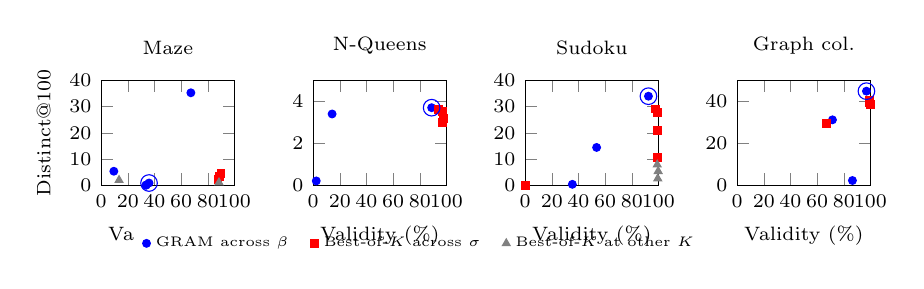
\begin{tikzpicture}
\begin{groupplot}[group style={group size=4 by 1, horizontal sep=1.0cm},
  width=0.27\textwidth, height=0.24\textwidth, xmin=0, xmax=100, ymin=0,
  xlabel={Validity (\%)}, tick label style={font=\scriptsize}, label style={font=\scriptsize},
  title style={font=\scriptsize}]
\nextgroupplot[title={Maze}, ylabel={Distinct@100}, ymax=40,
  legend style={font=\tiny, at={(2.4,-0.38)}, anchor=north, draw=none, legend columns=3,
    /tikz/every even column/.append style={column sep=6pt}}, legend cell align=left]
\addplot[only marks, mark=*, mark size=1.4pt, blue] coordinates {(9.5,5.3) (67.3,35.3) (35.9,0.8) (33.8,0.0) (33.6,0.0)};
\addplot[only marks, mark=square*, mark size=1.4pt, red] coordinates {(87.7,2.1) (88.5,3.2) (89.9,4.4)};
\addplot[only marks, mark=triangle*, mark size=1.6pt, black!50] coordinates {(88.4,1.0) (13.4,1.9)};
\legend{GRAM across $\beta$, \Bok{} across $\sigma$, \Bok{} at other $K$}
\addplot[only marks, mark=o, mark size=3pt, blue, forget plot] coordinates {(35.9,0.8)};
\nextgroupplot[title={N-Queens}, ymax=5]
\addplot[only marks, mark=*, mark size=1.4pt, blue] coordinates {(14.2,3.4) (88.9,3.7) (2.3,0.2)};
\addplot[only marks, mark=square*, mark size=1.4pt, red] coordinates {(97.1,3.0) (97.9,3.2) (97.3,3.5) (93.8,3.6)};
\addplot[only marks, mark=o, mark size=3pt, blue, forget plot] coordinates {(88.9,3.7)};
\nextgroupplot[title={Sudoku}, ymax=40]
\addplot[only marks, mark=*, mark size=1.4pt, blue] coordinates {(53.6,14.4) (92.5,34.0) (35.4,0.3)};
\addplot[only marks, mark=square*, mark size=1.4pt, red] coordinates {(99.2,10.4) (99.5,20.9) (99.5,27.7) (97.5,29.1) (0.0,0.0)};
\addplot[only marks, mark=triangle*, mark size=1.6pt, black!50] coordinates {(99.5,2.5) (99.8,5.3) (99.1,7.8)};
\addplot[only marks, mark=o, mark size=3pt, blue, forget plot] coordinates {(92.5,34.0)};
\nextgroupplot[title={Graph col.}, ymax=50]
\addplot[only marks, mark=*, mark size=1.4pt, blue] coordinates {(71.5,31.2) (97.0,44.9) (86.5,2.2)};
\addplot[only marks, mark=square*, mark size=1.4pt, red] coordinates {(99.8,38.4) (99.6,39.5) (99.4,40.4) (66.8,29.5)};
\addplot[only marks, mark=o, mark size=3pt, blue, forget plot] coordinates {(97.0,44.9)};
\end{groupplot}
\end{tikzpicture}
\caption{Validity against distinct@100 on validation inputs; up and to the right is better. Blue: GRAM at
$\frac12$, 1 and 2 times the reference $\beta$ (mazes: $\frac14$ to 4 times), with a ring at the reference $\beta$. Red: the
\bok{} baseline ($K=8$) with state noise $\sigma=0$, 0.25, 0.5, 1, 2 where run. Grey: the baseline at $K=1$, 4
(Sudoku) and 16 without state noise. Points from \cref{tab:beta,tab:noisefull,tab:k}. On every task, GRAM's best
$\beta$ and the baseline with state noise trade validity against distinct@100, and neither has both higher (on N-Queens GRAM leads by only 0.1--0.7, near the number of solutions).}
\label{fig:frontier}
\end{figure*}

\Cref{fig:frontier} puts both models on one plot per task. On every task GRAM at its best $\beta$ has the higher
distinct@100 and the baseline the higher validity, so neither model is better on both, and the answer to Q2 depends on
the use, as in \cref{tab:main}. What state noise changes is the size of the trade: on Sudoku the baseline gives up
5 points of distinct@100 to gain 5 points of validity, while at $\sigma=0$ it gave up 24.

\subsection{The usable $\beta$ is a narrow band}
\label{sec:band}

\begin{figure}[t]
\centering
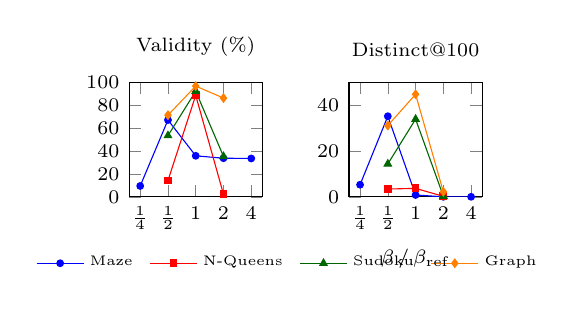
\begin{tikzpicture}
\begin{groupplot}[group style={group size=2 by 1, horizontal sep=1.1cm},
  width=0.27\textwidth, height=0.25\textwidth, xmode=log, log basis x=2,
  xtick={0.25,0.5,1,2,4}, xticklabels={$\frac14$,$\frac12$,1,2,4},
  xlabel={$\beta\,/\,\beta_{\mathrm{ref}}$}, tick label style={font=\scriptsize},
  label style={font=\scriptsize}, title style={font=\scriptsize}, ymin=0]
\nextgroupplot[title={Validity (\%)}, ymax=100,
  legend style={font=\tiny, at={(1.2,-0.42)}, anchor=north, draw=none, legend columns=4,
    /tikz/every even column/.append style={column sep=4pt}}, legend cell align=left]
\addplot[mark=*, mark size=1.2pt, blue] coordinates {(0.25,9.5) (0.5,67.3) (1,35.9) (2,33.8) (4,33.6)};
\addplot[mark=square*, mark size=1.2pt, red] coordinates {(0.5,14.2) (1,88.9) (2,2.3)};
\addplot[mark=triangle*, mark size=1.5pt, black!60!green] coordinates {(0.5,53.6) (1,92.5) (2,35.4)};
\addplot[mark=diamond*, mark size=1.5pt, orange] coordinates {(0.5,71.5) (1,97.0) (2,86.5)};
\legend{Maze, N-Queens, Sudoku, Graph}
\nextgroupplot[title={Distinct@100}, ymax=50]
\addplot[mark=*, mark size=1.2pt, blue] coordinates {(0.25,5.3) (0.5,35.3) (1,0.8) (2,0.0) (4,0.0)};
\addplot[mark=square*, mark size=1.2pt, red] coordinates {(0.5,3.4) (1,3.7) (2,0.2)};
\addplot[mark=triangle*, mark size=1.5pt, black!60!green] coordinates {(0.5,14.4) (1,34.0) (2,0.3)};
\addplot[mark=diamond*, mark size=1.5pt, orange] coordinates {(0.5,31.2) (1,44.9) (2,2.2)};
\end{groupplot}
\end{tikzpicture}
\caption{GRAM across $\beta$, relative to the reference $\beta_{\mathrm{ref}}$ (the authors' value; maze: our
pre-chosen 0.02). Every task degrades within a factor of two of its best $\beta$; the maze's best is half its
reference. Validation, run summaries.}
\label{fig:beta}
\end{figure}

We trained GRAM at half and twice each task's reference $\beta$, and on mazes at $\frac14$ to 4 times
(\cref{fig:beta}, \cref{tab:beta}). The baseline has no $\beta$; its one setting, $K$, is studied in
\cref{app:extra}. On every task, a factor of two in either direction from the best $\beta$ costs much
of its validity, its distinct@100 or both; graph colouring at half $\beta$ is the mildest case (validity 97 to 72\%,
distinct@100 45 to 31). We call the range of $\beta$ in which neither of the two failures below dominates the
\emph{band}; on every task it is narrower than a factor of two on each side. The failures on the two sides differ.
\begin{itemize}
  \item \textbf{Above the band: posterior collapse.} At twice the reference $\beta$ the training KL falls to
  $\sim$$10^{-3}$ or below (maze, graph colouring) and distinct@100 drops to 0--2.2. On mazes, Sudoku and graph
  colouring, unique-solution validity stays at 98--100\% while multi-solution inputs fail. On mazes at the reference
  $\beta$, already at this edge, 91\% of invalid samples are blended answers: every cell agrees with some stored
  solution but the answer matches none, as expected of a model trained on several targets without usable stochastic
  guidance. Posterior sampling confirms that the stochastic guidance carries nothing here: its validity equals prior
  sampling's (\cref{tab:posterior}). N-Queens is the exception: at twice its $\beta$ its unique-solution validity
  also falls (2.8\%), which blending does not explain, and posterior sampling fails too (1.7\%), so the network
  itself has stopped producing valid boards.
  \item \textbf{Below the band: prior--posterior mismatch.} At half the reference $\beta$, unique-solution validity
  also falls (N-Queens 7.7\%, mazes at $\frac14$: 9.3\%), although there is nothing to choose, and on N-Queens and
  graph colouring validity falls further as training continues (N-Queens: 47\% at 15k steps, 14\% at 150k). Yet
  posterior sampling is valid on 100\% of samples on N-Queens, Sudoku and graph colouring, and on 94\% of maze
  samples at a quarter of the reference $\beta$ (\cref{tab:posterior}). The network can decode valid answers; what
  fails is the stochastic guidance it gets at test time. We call this \emph{prior--posterior mismatch}: the
  posterior encodes the target in stochastic guidance that the prior does not produce, so prior sampling feeds the
  network values it was not trained on. The related ``holes problem'' of VAEs~\cite{rezende2018taming} concerns where
  the prior and the posteriors put probability mass; our term refers to what the network does with the two kinds of
  stochastic guidance, which posterior sampling measures directly.
\end{itemize}

\begin{table}[t]
\centering\footnotesize
\setlength{\tabcolsep}{4pt}
\begin{tabular}{@{}lccc@{}}
\toprule
Task & $\frac12\beta_{\mathrm{ref}}$ & $\beta_{\mathrm{ref}}$ & $2\beta_{\mathrm{ref}}$ \\
\midrule
Maze & 67.3 / 99.7 & 35.9 / 39.1 & 33.8 / 34.0 \\
N-Queens & 14.2 / 100.0 & 88.9 / 99.7 & 2.3 / 1.7 \\
Sudoku & 53.6 / 100.0 & 92.5 / 100.0 & 35.4 / 36.6 \\
Graph col. & 71.5 / 100.0 & 97.0 / 99.5 & 86.5 / 85.6 \\
\bottomrule
\end{tabular}
\caption{GRAM validity (\%) with prior sampling / posterior sampling, validation. Prior: run summaries; posterior:
final checkpoint. Below the band the posterior's stochastic guidance still gives valid answers; above it the two
agree, as expected when the stochastic guidance carries nothing.}
\label{tab:posterior}
\end{table}

\paragraph{A carried-over $\beta$ misses the band.} Mazes were the one task without an author setting, and the rule
that fits the authors' other puzzle settings ($\beta\times$cells $\approx 4.5$) placed it at the edge of posterior
collapse; its best value is half of that. Sudoku-Extreme's setting (0.1) also leads to posterior collapse on our Sudoku task. A $\beta$
that is right on one task is therefore not a safe starting point on another, which is the practical content of Q1.

\paragraph{The number of solutions varies within a task.} On mazes at $\beta=0.02$, GRAM's validity falls with the
number of solutions: 97.8\% at one, 48.4\% at 2--3, 19.2\% at 4--15, 1.9\% at 16--63 and 0\% above 64 (training
inputs; the baseline stays at 76--97\% in every group, \cref{tab:mazegroups}). Choosing one of $\Y$ solutions takes
about $\ln\Y$ nats of information in the stochastic guidance, so a single $\beta$ trades off differently for inputs
with 3 and with 300 solutions. This suggests replacing the global $\beta$ by a per-input information budget, which we
leave to the next version.

\subsection{Unseen solutions}

\begin{table}[t]
\centering\footnotesize
\setlength{\tabcolsep}{2.5pt}
\begin{tabular}{@{}lrcccc@{}}
\toprule
& & \multicolumn{2}{c}{Unseen share (\%)} & \multicolumn{2}{c}{Distinct unseen} \\
\cmidrule(lr){3-4}\cmidrule(l){5-6}
Task & Inputs & GRAM & BoK & GRAM & BoK \\
\midrule
Maze & 881 & 36.0 (38.5) & 75.7 (76.5) & 0.2 & 2.0 \\
Sudoku & 801 & 76.5 (76.6) & 77.0 (76.8) & 45.0 & 15.5 \\
Graph col. & 876 & 84.3 (84.5) & 84.7 (84.6) & 64.3 & 55.8 \\
\bottomrule
\end{tabular}
\caption{Training inputs with more than 16 solutions, final checkpoints, GRAM at the reference $\beta$ (maze 0.02),
BoK: \bok. Unseen share: valid samples that are unseen solutions; in parentheses, a uniform sampler's share. Distinct
unseen: per input, among 100 samples. N-Queens has only 14 such inputs (\cref{app:extra}).}
\label{tab:heldout}
\end{table}

On every task, both models produce unseen solutions at the rate a uniform sampler over the solution set would
(\cref{tab:heldout}): neither prefers its stored solutions. For Q2 this means that GRAM's posterior, which only ever
saw stored solutions, does not bias the prior towards them. GRAM's distinct unseen is higher where its distinct@100 is
higher overall (Sudoku, graph colouring).

\section{Related Work}

\paragraph{Recursive reasoning models.} HRM~\cite{wang2025hrm} and TRM~\cite{jolicoeur2025trm} solve puzzles with
small networks applied recursively. GRAM~\cite{baek2026gram} adds stochastic guidance with a learned prior and
posterior to produce several solutions. PTRM~\cite{sghaier2026ptrm} instead adds Gaussian noise to the low-level state
of a deterministic TRM at test time and returns the sample its halting head scores highest, and reports the accuracy of
that one answer rather than diversity.

\paragraph{Latent variable models.} The train/test mismatch of conditional VAEs and the ineffectiveness of raising
the KL weight were described by \citet{sohn2015cvae}, who proposed training partly on prior samples. Posterior
collapse~\cite{bowman2016generating} has many remedies, including free bits~\cite{kingma2016iaf}, $\beta$
schedules~\cite{higgins2017betavae} and $\delta$-VAEs~\cite{razavi2019delta}; none sets the information budget per
input from its number of solutions.

\paragraph{Learning with many solutions.} Multiple choice learning~\cite{guzmanrivera2012mcl} and its annealed
variant~\cite{perera2024amcl}, best-of-many~\cite{bhattacharyya2018bestofmany}, IMLE~\cite{li2018imle} and
one-of-many learning for combinatorial problems~\cite{nandwani2021oneofmany} train on the closest of several outputs
or targets. Our baseline is the simplest member of this family on GRAM's network.

\section{Limitations and Ongoing Work}
\label{sec:limits}

The main results are from one seed, on validation inputs, with 500 inputs per scored checkpoint. Second seeds on
Sudoku and mazes differ from the first by at most 5 points (\cref{app:extra}); second seeds on N-Queens and graph
colouring are training. Posterior sampling and state noise are measured on the final checkpoint only. The four tasks
are small and synthetic. The $\beta$ grid is coarse (factors of two). The maze row at $\beta=0.01$ is a tuned $\beta$,
chosen on the same validation inputs it is reported on. A fifth task, random 3-SAT, did not train for the baseline and
is excluded (\cref{app:sat}).

\section*{AI Use Statement}

An AI coding assistant was used substantially throughout this project: to write and debug training and evaluation
code, to analyse results, and to draft this manuscript. The authors designed the study, ran all experiments, checked
the reported numbers against the evaluation outputs and are responsible for the content.

\section*{Impact Statement}

This paper presents work whose goal is to advance the field of Machine Learning. There are many potential societal
consequences of our work, none which we feel must be specifically highlighted here.

\bibliography{refs}
\bibliographystyle{icml2027}

\newpage
\appendix
\onecolumn

\section{Benchmark Details}
\label{app:data}

\paragraph{Mazes.} A spanning-tree maze on a $7\times7$ lattice of rooms ($15\times15$ cells), with each remaining
inner wall removed with some probability to create loops, and a start and goal at least 8 cells apart along the maze. Any shortest
path is a valid answer; the number of shortest paths is counted exactly. Solution-count groups are $\log_2$-spaced.

\paragraph{N-Queens.} All 724 solutions of 10-Queens with 7, 8 or 9 queens removed; each distinct partial board is
one input and its completions are its solutions. Only 360 training inputs have more than 16 solutions and none more
than 93, so unseen-solution analyses on N-Queens rest on few inputs. The validation split is the first 1000 test
inputs, and final N-Queens test numbers will use the remaining 5{,}513.

\paragraph{Sudoku.} A random complete grid with 26--50 clues kept; puzzles with more than 1024 solutions are
discarded.

\paragraph{Graph 3-colouring.} A planted colouring of 10 nodes, with each pair of differently coloured nodes joined
with probability $p\sim U[0.1,1]$. Colourings are counted in canonical form (colours numbered by first appearance),
so two solutions differ in which nodes share a colour; the maximum, 9842, is the number of partitions of 10 nodes into
at most 3 groups.

\paragraph{Checks.} With the same checkers used for evaluation, every stored solution is valid and distinct, the
number stored equals $\min(\Y,16)$ on training inputs, and no input is shared between training and test or
validation.

\begin{table}[h]
\centering\small
\begin{tabular}{@{}lrrrrrrr@{}}
\toprule
& \multicolumn{6}{c}{Number of solutions} & Stored \\
\cmidrule(lr){2-7}
Dataset, split & 1 & 2--3 & 4--15 & 16--63 & 64--255 & 256+ & solutions \\
\midrule
Maze, train & 33{,}333 & 7{,}408 & 14{,}816 & 14{,}815 & 14{,}814 & 14{,}814 & 885{,}729 \\
N-Queens, train & 13{,}586 & 15{,}427 & 7{,}534 & 293 & 67 & 0 & 102{,}513 \\
Sudoku, train & 33{,}333 & 13{,}334 & 13{,}334 & 13{,}333 & 13{,}333 & 13{,}333 & 800{,}363 \\
Graph col., train & 33{,}333 & 11{,}112 & 11{,}111 & 11{,}111 & 11{,}111 & 22{,}222 & 850{,}425 \\
\bottomrule
\end{tabular}
\caption{Training inputs per group of solution counts.}
\end{table}

\section{Additional Results}
\label{app:extra}

\begin{table}[h]
\centering\small
\begin{tabular}{@{}llccccl@{}}
\toprule
Task & $\beta$ & Validity & Unique-sol.\ validity & Distinct@100 & Coverage@10 & Training KL (end) \\
\midrule
Maze & 0.005 & 9.5 & 9.3 & 5.3 & & \\
 & 0.01 & 67.3 & 48.2 & 35.3 & & \\
 & 0.02 & 35.9 & 97.8 & 0.8 & & 0.1--0.5 \\
 & 0.04 & 33.8 & 98.6 & 0.0 & & $\sim$0.001 \\
 & 0.08 & 33.6 & 99.3 & 0.0 & & $\sim$0.0003 \\
\midrule
N-Queens & 0.0225 & 14.2 & 7.7 & 3.4 & 0.42 & \\
 & 0.045 & 88.9 & 79.9 & 3.7 & 0.89 & \\
 & 0.09 & 2.3 & 2.8 & 0.2 & 0.04 & \\
\midrule
Sudoku & 0.025 & 53.6 & 79.8 & 14.4 & & \\
 & 0.05 & 92.5 & 97.6 & 34.0 & & \\
 & 0.1 & 35.4 & 98.3 & 0.3 & & \\
\midrule
Graph col. & 0.225 & 71.5 & 93.4 & 31.2 & & 3.4 \\
 & 0.45 & 97.0 & 97.4 & 44.9 & & \\
 & 0.9 & 86.5 & 100.0 & 2.2 & & 0.0004 \\
\bottomrule
\end{tabular}
\caption{GRAM across $\beta$ (validation, run summaries; coverage@10 at the final checkpoint). Training KL is the KL
term before multiplying by $\beta$, read off the training curves; blank where not read.}
\label{tab:beta}
\end{table}

\begin{table}[h]
\centering\small
\begin{tabular}{@{}lcccccc@{}}
\toprule
Maze solutions & 1 & 2--3 & 4--15 & 16--63 & 64--255 & 256+ \\
\midrule
Inputs & 660 & 144 & 300 & 299 & 297 & 300 \\
GRAM, $\beta=0.02$ & 97.8 & 48.4 & 19.2 & 1.9 & 0.1 & 0.0 \\
\Bok & 75.9 & 79.2 & 90.9 & 97.0 & 97.0 & 95.2 \\
\bottomrule
\end{tabular}
\caption{Maze validity (\%) by number of solutions, first 2000 training inputs, final checkpoints.}
\label{tab:mazegroups}
\end{table}

\begin{table}[h]
\centering\small
\begin{tabular}{@{}llcccc@{}}
\toprule
Task & & $K=1$ & $K=4$ & $K=8$ & $K=16$ \\
\midrule
& Inputs per optimiser step & 768 & 192 & 96 & 48 \\
\midrule
Sudoku & Validity & 99.5 & 99.8 & 99.2 & 99.1 \\
 & Unique-sol.\ validity & 99.8 & & 99.3 & \\
 & Distinct@100 & 2.5 & 5.3 & 10.4 & 7.8 \\
 & Distinct@100, state noise $\sigma=0.5$ & 18.0 & & 27.7 & \\
\midrule
Maze & Validity & 88.4 & & 83.3 & 13.4 \\
 & Unique-sol.\ validity & 94.1 & & 75.4 & 20.5 \\
 & Distinct@100 & 1.0 & & 2.2 & 1.9 \\
\bottomrule
\end{tabular}
\caption{The baseline across $K$ at matched compute (validation, run summaries; state noise: final checkpoint).
$K=1$ is MinLoss alone. Blank: not run.}
\label{tab:k}
\end{table}

\paragraph{Number of rollouts.} On Sudoku (\cref{tab:k}), validity stays at 99\% from $K=1$ to $K=16$, and
distinct@100 rises from 2.5 at $K=1$ to 10.4 at $K=8$; trained twice as long, $K=16$ reaches 12.9 (300k optimiser
steps, validity 98.6\%). The best-of-$K$ objective therefore adds diversity that MinLoss alone does not have, and
state noise adds about the same amount on top of either ($+15.5$ at $K=1$, $+17.3$ at $K=8$). On mazes, larger $K$
lowers validity, most of all on unique-solution inputs (94\% at $K=1$, 75\% at $K=8$), and $K=16$ fails: its validity
reached 74\% at 33k optimiser steps, then fell to 9--17\% for the rest of training, on inputs with any number of
solutions (5--21\% in every group). Since $K$ also sets the number of inputs per optimiser step (768 at $K=1$, 48 at
$K=16$), these runs do not tell whether the cause is the number of rollouts or the smaller number of inputs behind each
optimiser step. A second seed of $K=16$ is training.

\begin{table}[h]
\centering\small
\begin{tabular}{@{}lccccc@{}}
\toprule
State noise $\sigma$ & 0 & 0.25 & 0.5 & 1 & 2 \\
\midrule
Maze & 87.7 / 2.1 & & 88.5 / 3.2 & 89.9 / 4.4 & \\
N-Queens & 97.1 / 3.0 & & 97.9 / 3.2 & 97.3 / 3.5 & 93.8 / 3.6 \\
Sudoku & 99.2 / 10.4 & 99.5 / 20.9 & 99.5 / 27.7 & 97.5 / 29.1 & 0.0 / 0.0 \\
Graph col. & 99.8 / 38.4 & & 99.6 / 39.5 & 99.4 / 40.4 & 66.8 / 29.5 \\
\bottomrule
\end{tabular}
\caption{Validity (\%) / distinct@100 of the \bok{} baseline ($K=8$) with state noise, validation; $\sigma>0$ on the
final checkpoint, $\sigma=0$ as in \cref{tab:noise}. Blank: not run.}
\label{tab:noisefull}
\end{table}

\paragraph{State noise.} Distinct@100 rises with $\sigma$ until validity breaks, at $\sigma=2$ on Sudoku and graph
colouring (\cref{tab:noisefull}). On GRAM at Sudoku's reference $\beta$, $\sigma=0.5$ gives validity 91.2\%,
unique-solution validity 97.2\% and distinct@100 33.7, against 92.5\%, 97.6\% and 34.0 without it.

\begin{table}[h]
\centering\small
\begin{tabular}{@{}llcc@{}}
\toprule
Task & Model & Seed 1 & Seed 2 \\
\midrule
Sudoku & GRAM, $\beta=0.05$ & 92.5 / 97.6 / 34.0 & 93.1 / 98.0 / 34.4 \\
 & \Bok, $K=8$ & 99.2 / 99.3 / 10.4 & 99.2 / -- / 9.4 \\
Maze & GRAM, $\beta=0.01$ (tuned) & 67.3 / 48.2 / 35.3 & 62.6 / 44.6 / 36.2 \\
\bottomrule
\end{tabular}
\caption{Two training seeds: validity (\%) / unique-solution validity (\%) / distinct@100, validation, run summaries.
Second seeds of the other rows are training.}
\label{tab:seeds}
\end{table}

\paragraph{Seeds.} Runs that differ only in the training seed differ by at most 1 point on Sudoku and by 5 points of
validity on mazes at $\beta=0.01$ (\cref{tab:seeds}), smaller than the differences between methods and between
values of $\beta$ that we report.

\paragraph{Ratio to uniform.} For reference, the ratios at the reference $\beta$ (validation, run summaries) are: maze
0.84 (GRAM) and 0.14 (\bok), N-Queens 1.00 and 0.86, Sudoku 0.97 and 0.44, graph colouring 0.96 and 0.81. GRAM's
ratios are close to 1 on every task; on mazes this reflects its few valid samples rather than diversity.

\paragraph{N-Queens unseen solutions.} On the 14 training inputs with more than 16 solutions, the unseen share is
35.5\% for GRAM and 38.7\% for \bok, against 35.3\% and 35.6\% for a uniform sampler.

\paragraph{Training dynamics.} The baseline's distinct@100 on Sudoku and graph colouring first falls as validity
rises and then recovers; GRAM at $\beta=0.01$ on mazes swings between 4\% and 76\% validity across checkpoints. The
second GRAM seeds dip and recover too: on mazes validity stays at 46--51\% until 60k optimiser steps and then reaches
60--68\%, and on Sudoku it drops to 71\% at 75k optimiser steps between checkpoints at 90\% and 93\%.

\section{Random 3-SAT}
\label{app:sat}

A fifth benchmark of random 3-SAT formulas over 16 variables (clause density $U[1,4.5]$, up to a quarter of the
variables given) was built the same way. The baseline did not learn it: 0.4\% of its samples were valid after 50k
optimiser steps, close to random assignments, and its training loss rose during training. GRAM failed the same way in
an earlier configuration. We exclude the task until the cause is understood.

\end{document}
